\section{Dataset}

In this investigation, we will utilize the Modified National Institute of Standards and Technology (MNIST) dataset \cite{lecun-mnisthandwrittendigit-2010}, which is widely recognized as a benchmark for image classification tasks. The dataset comprises $60,000$ \textit{training} images and $10,000$ \textit{testing} images, each representing a handwritten digit in grayscale and measuring 28x28 pixels. Consequently, there are ten unique classes, each corresponding to a different digit. An example of the images is shown in \Fig~\ref{fig:mnist}.

\begin{figure}[h]
	\centering
	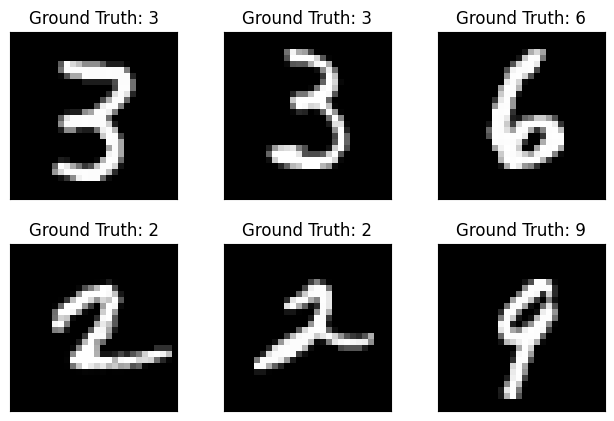
\includegraphics[width=0.5\linewidth]{ImageFiles/Dataset/mnist}
	\caption{Example images from the MNIST dataset}
	\label{fig:mnist}
\end{figure}

In this work, the training set is further divided into two parts. Specifically, $40,000$ images are used for training the model, while the remaining $10,000$ images are utilized for validation purposes. This approach allows for better monitoring and tuning of the model architecture and hyperparameters during the training process. The  same data partitioning scheme is employed for both networks.